\chapter{Experimental evaluation}
\label{06:chapter:title}

This chapter is devoted to testing and experimentally evaluating of proposed parallel execution designed and implemented in
Chapters~\ref{04:chapter:title},~\ref{05:chapter:title}.
In addition, we designed experiments to prove the parallelism we created scales (i.e., method or class-wide).
At the same time, we calculated Amhdal's law for each experiment and compared it with the achieved result.

\section{Experiments design}

The overall design of the experiments is divided into three main categories;
(a) preliminary experiments to prove that the parallelization we propose is capable of vertical scaling.
These experiments will be performed for small Kubernetes instances (i.e., Minikube) and multi-node Kubernetes clusters.
The expected results should be positive because parallelization will have the best possible implementation environment
(f.e., for method-wide parallelization, it will be a test class containing only tests that are capable of parallel computation,
similarly to class-wide parallelization.);
(b) the next part will be acceptance experiments, which will primarily provide information on whether it is beneficial
to use parallelization in a small subset of tests, where mostly half of the tests are capable of parallel execution.
Acceptance experiments will include a subset of our system of tests, where of course, there will also be tests and test classes,
which are not capable of parallel execution, and thus synchronization will occur.
Possibly the parallelization will not be suitable for acceptance experiments because most test suites consist of one or two test cases,
and the overall preparation phase of the test suite is long.;
(c) last type of experiments will be the so-called regression, which will already include the entire test suite currently offered by the Strimzi project.
It will tell us whether the given parallelization is eligible for the Strimzi.
Moreover, a significant acceleration is expected because test classes often contain ten or more tests.
On the other hand, we also have many tests that need total isolation, which potentially can slow down the whole performance.

We mainly use the Openstack and Amazon Web Services infrastructures to perform all the experiments, which will provide us with the necessary hardware resources.
Furthermore, for preliminary experiments, we use four types of instances:
\begin{itemize}
    \item \textbf{Kubernetes cluster} \---\ multi-node, where this instance will provide 24 virtual cores and 48 GB RAM (without taking into account master nodes)
    \item \textbf{Small minikube} \---\ single-node, where this instance will provide two virtual cores and 8GB RAM
    \item \textbf{Medium minikube} \---\ single-node, where this instance will provide four virtual cores and 16GB RAM
    \item \textbf{Large minikube} \---\ single-node, where this instance will provide eight virtual cores and 32GB of RAM
\end{itemize}

\section{Preliminary experiments}

Recall~\ref{04:amdalhlaw} Amdahl's formula from Chapter~\ref{03:chapter:title}.
We will not count the unit of work as the number of tests capable of parallel execution, but we will use a more accurate way (i.e., execution time).
We also introduce a new formula~\eqref{eqn:t-new-formula}, which also calculates the theoretical time after acceleration and then, thanks to this
the result, we calculate the total possible acceleration using the formula~\eqref{eqn:acc-formula}.
All markings are the same as described in Chapter~\ref{03:chapter:title} under Amdahl's law;
we have $T_{new}$ and $T_{old}$. $T_{old}$ describes the time necessarily performed (i.e., sequentially) by a given task.
On the other hand, $T_{new}$ describes the time after acceleration Equation~\eqref{eqn:t-new-formula}

\begin{equation}
    \label{eqn:t-new-formula}
    T_{new} = (1 - p) * T_{old} +  \frac{p}{s} * T_{old}
    \tag{4}
\end{equation}

\begin{equation}
    \label{eqn:acc-formula}
    S = \frac{T_{old}}{T_{new}}
    \tag{5}
\end{equation}

In the case of our experiment, we have the test class \textbf {SecurityST}, which includes twenty-one test cases.
All these tests can be performed in parallel and are a perfect candidate to obtain information that parallelization is capable of vertical scaling.
What should be noted is the fact that the shared Cluster Operator is deployed before the execution tests,
where usually this deployment lasts from one to six minutes (we choose a mean value of three minutes).
So in our case, the part that can be parallelized will be equal to $p = \frac{171}{174}$.
The first instance we use is a multi-node Kubernetes cluster with 24 virtual cores and 48 GB of RAM.
Empirically, we obtained data on how long it takes to complete a given test class sequentially, using such information in Amdahl's law.
\begin{equation}
    \label{eqn:security-st-time-ocp}
    T_{new} = (1 - \frac{171}{174}) * 174 +  \frac{\frac{171}{174}}{24} * 174 =~10~minutes
    \tag{6}
\end{equation}
In Equation~\eqref{eqn:security-st-time-ocp}, one can see the theoretical time we should approach in first experiments executing \textbf{SecurityST} test suite.
Furthermore, the entire acceleration could be up to 17 times (i.e, Equation~\eqref{eqn:prelim-method-wide}).
Of course, we know from practice that we will not get exactly such an acceleration;
we can solely get nearer to it.
\begin{equation}
    \label{eqn:prelim-method-wide}
    S = \frac{174}{10} =17.4x
    \tag{7}
\end{equation}
Additionally, we use the following notation in the tables:
\begin{itemize}[itemsep=1mm, parsep=0pt]
    \item {\xmark} \---\ disabled parallelism (f.e., method or class-wide), or test execution containing errors (f.e., cluster crashed, because of out of memory problem)
    \item {\cmark} \---\ enabled parallelism (f.e., method or class-wide), or test execution without any issues
    \item {\fontencoding{U}\fontfamily{futs}\selectfont\char 66\relax} \---\ test execution with flaky tests because of resource capacity
\end{itemize}

In the following Table~\ref{06:tab:01:securityst-ocp-multinode}, we can see the individual preliminary experiments performed over our implementation.
For clarity, a sequential variant is also included.
We slowly increased the threads used to determine if a given parallelization scales there (i.e., we started from two to sixteen).
As part of our experimentation, we found that up to twelve threads would be the best candidate for \textbf{SecurityST}.
As shown in Table~\ref{06:tab:01:securityst-ocp-multinode}, when using sixteen threads, the given Kubernetes cluster was destroyed.
The reason was mainly the capacity resources (i.e., we deploy Kafka cluster and many other resources for each test case).
At the same time, we can notice that we did not reach the theoretical acceleration that we calculated in Equation~\eqref{eqn:security-st-time-ocp}.
However, this is due to several factors (f.e., tests do not take the same time or slower deployment volumes within Kafka clusters).
Nevertheless, one needs to realize that if we had hypothetically unlimited resources (i.e., cores, RAM), we would not be able to overcome
the acceleration we calculated (i.e., Equation~\eqref{eqn:amdalh-limit}).
\begin{table}[ht!]
    \centering
    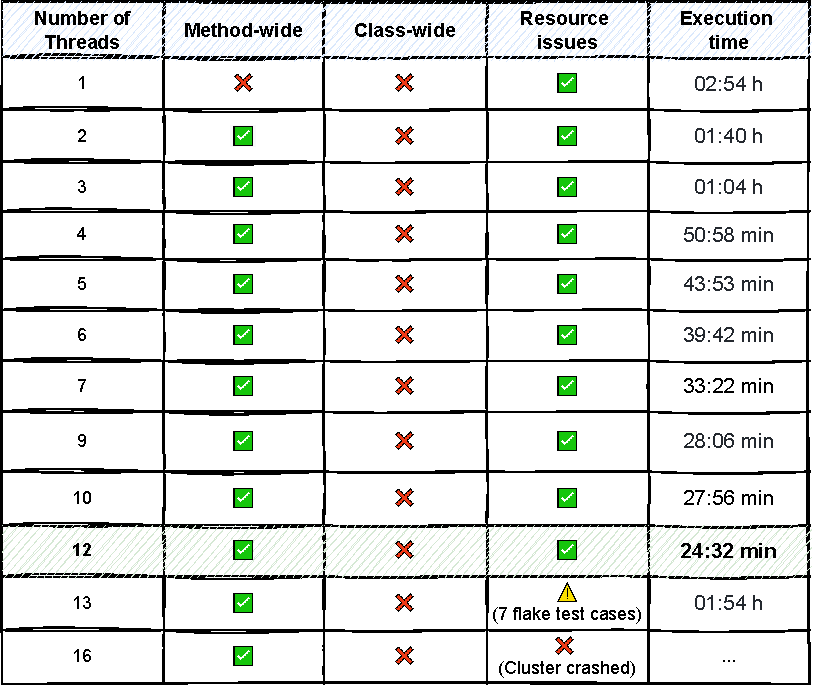
\includegraphics[scale=0.8]{obrazky-figures/08-experiments/06-exp-final-smoke-method-wide-ocp}
    \caption{The \textbf{SecurityST} contains twenty-one test cases, and all of them could be executed in parallel
        (i.e., contains @ParallelTest or @ParallelNamespaceTest annotation).
        Moreover, each test case deploys a Kafka cluster, which perfectly verifies if the Kubernetes cluster
        or Minikube (i.e., single-node) can handle such a load.}
    \label{06:tab:01:securityst-ocp-multinode}
\end{table}

\begin{equation}
    \label{eqn:amdalh-limit}
    \lim_{s\to\infty} S_{max} = \frac{1}{1-p} = \frac{1}{1-\frac{171}{174}} = 58x
    \tag{8}
\end{equation}
Our acquired acceleration in a perfect environment is less than $S _{\max} = 58x$ and at the same time $S_{teo} = 17.4x$.
However, this is confirmed by the fact that we will never be better than $S_{\max}$ and also, we will never achieve a
possible theoretical acceleration (i.e., $S_{teo}$) because such results are entirely typical for this kind of experiments.
Overall, our acceleration is $S_{practical} = \frac{174}{24.5} = 7.1x$, which proves following relation $S_{practical} < S_{teo} < S_{\max}$.

%---------------------------------------------------------
%--------------------MINIKUBE PART------------------------
%---------------------------------------------------------

Other preliminary experiments we performed were on more minor instances where it was a matter of course that the results
accelerations compared to a multi-node cluster will be significantly lower and slower.
Therefore, Amdalh's law will also contain a much lower theoretical acceleration.
For a machine containing four virtual cores, the estimated theoretical time is $T_{new\_teo\_medium}$, which is equal to
$T_{new\_teo\_medium} = (1 - \frac{182}{185}) * 185 + \frac{\frac{182}{185}} {4} * 185 = $ approximately 49~minutes.
So the theoretical acceleration of the instance could be $S_{new\_teo\_medium} = \frac{185}{49} = 3.8x$.
Nevertheless, as we can see in Table~\ref{06:tab:01:securityst-minikube}, we did not accomplish such a same acceleration.
However, we have come close enough, and the practical acceleration is $S_{new\_practical\_medium} = \frac{185}{79} = 2.34x$.
We could use a maximum of three cores because, in the case of four cores, the virtual machine crashes due to a lack of memory.
CPU utilization was approximately 80\% during the use of the four cores.
\begin{table}[ht!]
    \centering
    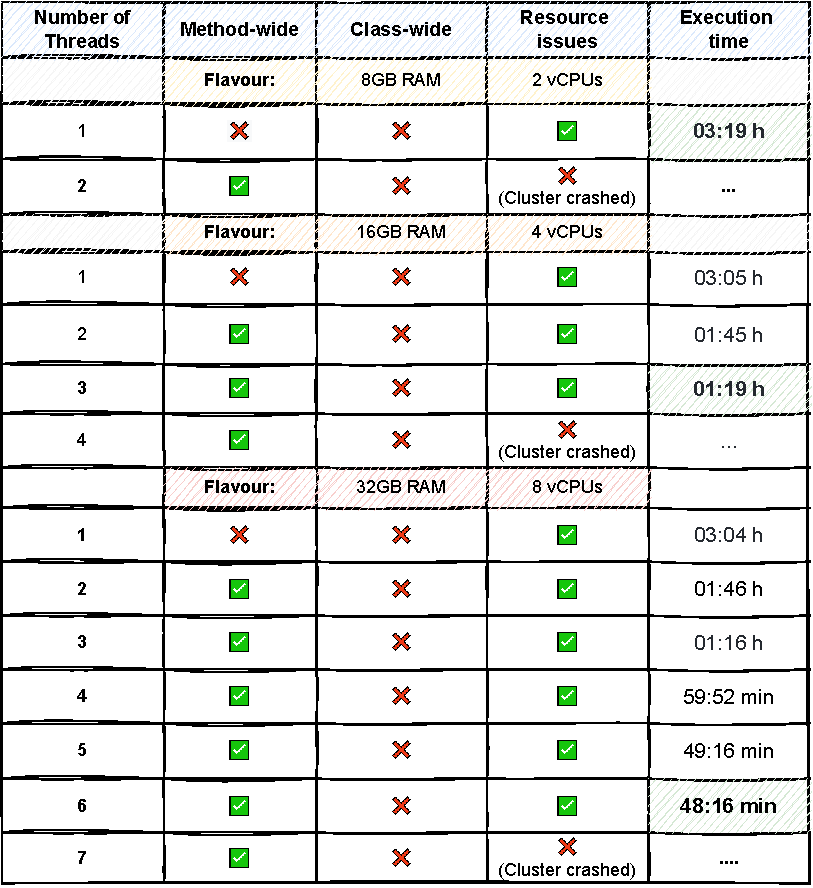
\includegraphics[scale=0.8]{obrazky-figures/08-experiments/06-exp-preliminary-minikube-b}
    \caption{Multiple experiments for various flavours of single-node Kubernetes instances for the
    \textbf{SecurityST} suite. Both of these flavours (i.e., orange and red one prove that parallelisation is
    vertically scaling on more minor instances), the yellow one (i.e., using two virtual cores and eight GB RAM)
        is not able to run either two test cases in parallel resulting in OOM problem (i.e., Out of memory).}
    \label{06:tab:01:security-st-minikube}
\end{table}
%-------------------------------------------------------
%-------b) PRELIMINARY EXPERIMENTS FOR CLASS-WIDE-------
%-------------------------------------------------------

Dalšie experimenty, ktoré majú dokázať, že nami implementovaná class-wide parallelizácia je možná vertikálneho škálovania.
Preto sme vybrali množinu testovacích tried, ktoré nepotrebujú žiadnu formu sychronizácie alebo izolácie (i.e., neobsahujú @IsolatedSuite anotáciu).
Špecificky sa bude jednať o triedy obsahujúce anotáciu @ParallelSuite a nimi sú práve HttpBridgeScramShaST, HttpBridgeTlsST,
ThrottlingQuotaST, TopicST, UserST, ReconciliationST a CruiseControlConfigurationST. Spolu obsahujú tridsať testovacích
prípadov, kde celkovo 29 nepotrebujú žiadnu formu sychronizácie a iba 1 testovací prípad potrebuje izoláciu voči ostatným testom.
Presnejšie máme 10 @ParallelNamespaceTest, pre zopakonie sú to testy ktoré deploynú Kafka cluster a teda sa radia medzi
viac resource náročné.
Ďalej máme 19 @ParallelTest taktiež možno povedať lighweight variantou na potrebu celkových zdrojov a nakoniec jeden @IsolatedTest
zaručújúci izolácia od ostatných parallelných testov.
V prípade ak by sme chceli vypočívať možné teoretické zrýchlenie tak je nutné poznať sekvenčný čas a zároveň tak čas jedného @IsolatedTest.
Celkový čas nami vybraními testovami je 107~minút a z toho @IsolatedTest trvá 2.5 minúty.
Ak k tomu pripočítame preparačný čas zdieľaného Cluster Operatora tak sa dostaneme na 5.5 minúty a teda možná paralelná čas bude rovná $p = \frac{101.5}{107}$.
Speedup factor je rovný počtu virtual CPU, ktoré máme k dispozící (i.e., $S=24$) a vďaka tomu može všetky hodnoty dosadiť do
vzorca nadefinovaného vyššie (i.e., Equation~\eqref{eqn:t-new-formula}).
\begin{equation}
    \label{eqn:class-wide-time-ocp}
    T_{new} = (1 - \frac{101.5}{107}) * 107 +  \frac{\frac{101.5}{107}}{24} * 107 =~10~minutes
    \tag{6}
\end{equation}
Po vypočítaní nám vyjde, že teoretické zrýchlenie pri použítí 24 jadier sa bude blížiť ku 10 minútam z čoho si zároveň
možeme vypočítať aj $S_{teo} = \frac{T_{old}}{T_{new}} = \frac{107}{10} =~10.7x$ a $\lim_{s\to\infty} S_{\max} = \frac{1}{1-p} = \frac{1}{1-\frac{101.5}{107}} =~19x$.

Čo je nutné podotknúť je, že pre class-wide parallelizáciu je najlepším možným scenárom máť konzistentné rozloženie testov
najideálnejśie podporujú parallelnú exekúciu (f.e., mať 5 testovacích tried, ktoré každá z nich obsahuje 10 parallel testov).
Tým za získa z daného typu parallelizácie najviac.
Triedy, ktoré sme využili avšak neposkytujú presne také rovnomerné rozloženie čo je zároveň aj v praxi takmer nemožné
(i.e, mať rovnaký počet testov pre každú testovaciu triedu).

Experimenty, ktoré sme vykonali je možné vidieť v Tabuľke~\ref{06:tab:01:class-widesecurityst-ocp} obdobne ako pre method-wide
parallelizáciu sme najskôr dodali totálne sekvenčné vykonanie a následne sme pridávali vlákna.
Zároveň sme aj v rámci experimentoch porovnali vykonávanie method-wide (i.e., orange row color), kde celkové vykonávanie trvalo
podstatne viac ako v prípade class-wide parallelizácie (i.e, green row color).
Hlavným dôvodom prečo pri využítí 10 vlákien class-wide parallelizácia bola o viac než pol hodinu lepšia bola kvoli tomu, že
nie v každej testovacej triede bolo testov väčší ako 10 a teda v method-wide parallelizácií sa použílo zbytočne veľa vlákien,
ktoré sa vlastne nevyužili.
Na druhú stranu class-wide parallelízícia 10 vlákien plne využila, pretože može vykonávať viacero tried zároveň a tým podstatne zvýšiť celkový čas.

% HttpBridgeScramShaST - 2 parallel test                  = 2
% HttpBridgeTlsST - 2 parallel test                       = 2
% ThrottlingQuotaST - 4 parallel test                     = 4
% TopicST - 5 parallel test a 1 isolated                  = 6 (1 isolated)
% UserST - 6 parallel test a 2 Paralle namespace test     = 8
% ReconciliationST - 2 parallel namespace test            = 2
% CruiseControlConfigurationST - 6 parallel namespace test= 6
% ----
% 10 PNT, 19 PT a 1 IT

\begin{table}[ht!]
    \centering
    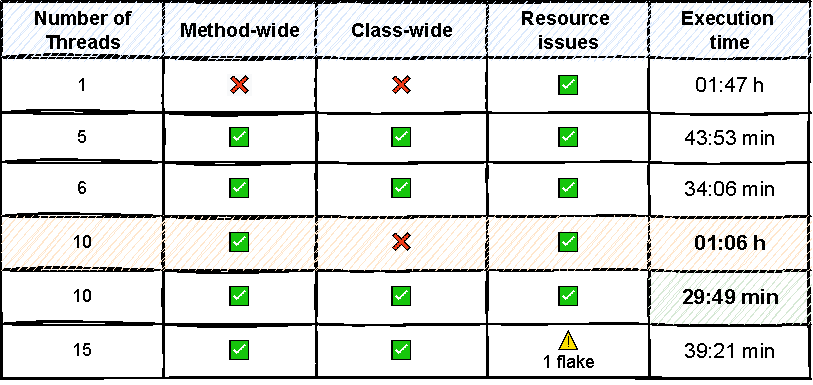
\includegraphics[scale=0.8]{obrazky-figures/08-experiments/06-exp-preliminary-cluster-wide-ocp}
    \caption{Preliminary experiments with Security test suite containing twenty-one test cases, which all can be run in parallel.
    Each test case deploys Kafka cluster, which perfectly verifies if Kubernetes cluster or Minikube (i.e., single-node) can handle such a load.}
    \label{06:tab:01:class-widesecurityst-ocp}
\end{table}

%-------------------------------------------------------------
%------------- END OF PRELIMINARY EXPERIMENTS ----------------
%-------------------------------------------------------------

\section{Acceptance experiments}

Tento typ experimentov bude zahrnovať nášu reálnu podmnožinu testov, ktorá sa vykonávana ako jedna z príslušných jobov v CI
nástroji. Výsledok týchto testov nám zároveň dodá informáciu, či je ideálne púštať paralelne. Kedže viem, že daný profil
obsahuje aj dosť testov pre ktoré je nutná izoláciu (i.e., @IsolatedTest) a rovnako tak aj testovacie triedy (i.e., @IsolatedSuite).
V tomto ohlade sa teda čaká podstatne slabšie zrýchlenie ak to porovnáme z preliminárnymi experimentami, ktoré sa púštali
s takmer najlepšom prostredí pre paralelizáciu. Zároveň kedže sme zistili, že flavour \emph{2CPUs a 8GB RAM}, nie je
možný vykonávať ani dve paralelné testy a teda je pre tento typ experimentu zbytočný.

\subsection{Method-wide}

Ako minule začneme

acceptance profile...

\section{Regression experiments}

regression profile...

\chapter{Future work}
\label{07:chapter:title}

\chapter{Conclusion}
\label{08:chapter:title}

